\documentclass[12pt,spanish]{article}
\usepackage[spanish]{babel}
\selectlanguage{spanish}
\usepackage[utf8x]{inputenc}
\usepackage{graphicx}
\graphicspath{{images/}}
\usepackage{amsfonts}
\usepackage{float}
\usepackage{url}
\usepackage{fancyhdr}
\usepackage{vmargin}
\usepackage{multirow}
\usepackage{chngpage}
\usepackage{hyperref}

\usepackage{subcaption}

\usepackage[
    type={CC},
    modifier={by-nc-sa},
    version={4.0},
]{doclicense}

\hypersetup{
    colorlinks=true,
    linkcolor=blue,
    filecolor=magenta,
    urlcolor=cyan,
}

% para codigo
\usepackage{listings}
\usepackage{xcolor}



%% configuración de listings

\definecolor{listing-background}{HTML}{F7F7F7}
\definecolor{listing-rule}{HTML}{B3B2B3}
\definecolor{listing-numbers}{HTML}{B3B2B3}
\definecolor{listing-text-color}{HTML}{000000}
\definecolor{listing-keyword}{HTML}{435489}
\definecolor{listing-identifier}{HTML}{435489}
\definecolor{listing-string}{HTML}{00999A}
\definecolor{listing-comment}{HTML}{8E8E8E}
\definecolor{listing-javadoc-comment}{HTML}{006CA9}

\lstdefinestyle{eisvogel_listing_style}{
  language         = python,
%$if(listings-disable-line-numbers)$
%  xleftmargin      = 0.6em,
%  framexleftmargin = 0.4em,
%$else$
  numbers          = left,
  xleftmargin      = 0em,
 framexleftmargin = 0em,
%$endif$
  backgroundcolor  = \color{listing-background},
  basicstyle       = \color{listing-text-color}\small\ttfamily{}\linespread{1.15}, % print whole listing small
  breaklines       = true,
  frame            = single,
  framesep         = 0.19em,
  rulecolor        = \color{listing-rule},
  frameround       = ffff,
  tabsize          = 4,
  numberstyle      = \color{listing-numbers},
  aboveskip        = 1.0em,
  belowskip        = 0.1em,
  abovecaptionskip = 0em,
  belowcaptionskip = 1.0em,
  keywordstyle     = \color{listing-keyword}\bfseries,
  classoffset      = 0,
  sensitive        = true,
  identifierstyle  = \color{listing-identifier},
  commentstyle     = \color{listing-comment},
  morecomment      = [s][\color{listing-javadoc-comment}]{/**}{*/},
  stringstyle      = \color{listing-string},
  showstringspaces = false,
  escapeinside     = {/*@}{@*/}, % Allow LaTeX inside these special comments
  literate         =
  {á}{{\'a}}1 {é}{{\'e}}1 {í}{{\'i}}1 {ó}{{\'o}}1 {ú}{{\'u}}1
  {Á}{{\'A}}1 {É}{{\'E}}1 {Í}{{\'I}}1 {Ó}{{\'O}}1 {Ú}{{\'U}}1
  {à}{{\`a}}1 {è}{{\'e}}1 {ì}{{\`i}}1 {ò}{{\`o}}1 {ù}{{\`u}}1
  {À}{{\`A}}1 {È}{{\'E}}1 {Ì}{{\`I}}1 {Ò}{{\`O}}1 {Ù}{{\`U}}1
  {ä}{{\"a}}1 {ë}{{\"e}}1 {ï}{{\"i}}1 {ö}{{\"o}}1 {ü}{{\"u}}1
  {Ä}{{\"A}}1 {Ë}{{\"E}}1 {Ï}{{\"I}}1 {Ö}{{\"O}}1 {Ü}{{\"U}}1
  {â}{{\^a}}1 {ê}{{\^e}}1 {î}{{\^i}}1 {ô}{{\^o}}1 {û}{{\^u}}1
  {Â}{{\^A}}1 {Ê}{{\^E}}1 {Î}{{\^I}}1 {Ô}{{\^O}}1 {Û}{{\^U}}1
  {œ}{{\oe}}1 {Œ}{{\OE}}1 {æ}{{\ae}}1 {Æ}{{\AE}}1 {ß}{{\ss}}1
  {ç}{{\c c}}1 {Ç}{{\c C}}1 {ø}{{\o}}1 {å}{{\r a}}1 {Å}{{\r A}}1
  {€}{{\EUR}}1 {£}{{\pounds}}1 {«}{{\guillemotleft}}1
  {»}{{\guillemotright}}1 {ñ}{{\~n}}1 {Ñ}{{\~N}}1 {¿}{{?`}}1
  {…}{{\ldots}}1 {≥}{{>=}}1 {≤}{{<=}}1 {„}{{\glqq}}1 {“}{{\grqq}}1
  {”}{{''}}1
}
\lstset{style=eisvogel_listing_style}


\usepackage[default]{source sans pro}

\setmarginsrb{2 cm}{1 cm}{2 cm}{2 cm}{1 cm}{1.5 cm}{1 cm}{1.5 cm}
\title{Práctica 1:\\
Máscaras y derivadas  \hspace{0.05cm} }
\author{Ángel Cabeza Martín}
\date{\today}

\renewcommand*\contentsname{hola}

\makeatletter
\let\thetitle\@title
\let\theauthor\@author
\let\thedate\@date
\makeatother

\pagestyle{fancy}
\fancyhf{}
\rhead{\theauthor}
\lhead{\thetitle}
\cfoot{\thepage}

\begin{document}

%%%%%%%%%%%%%%%%%%%%%%%%%%%%%%%%%%%%%%%%%%%%%%%%%%%%%
\begin{titlepage}
 
 
\newlength{\centeroffset}
\setlength{\centeroffset}{-0.5\oddsidemargin}
\addtolength{\centeroffset}{0.5\evensidemargin}
\thispagestyle{empty}

\noindent\hspace*{\centeroffset}

\centering
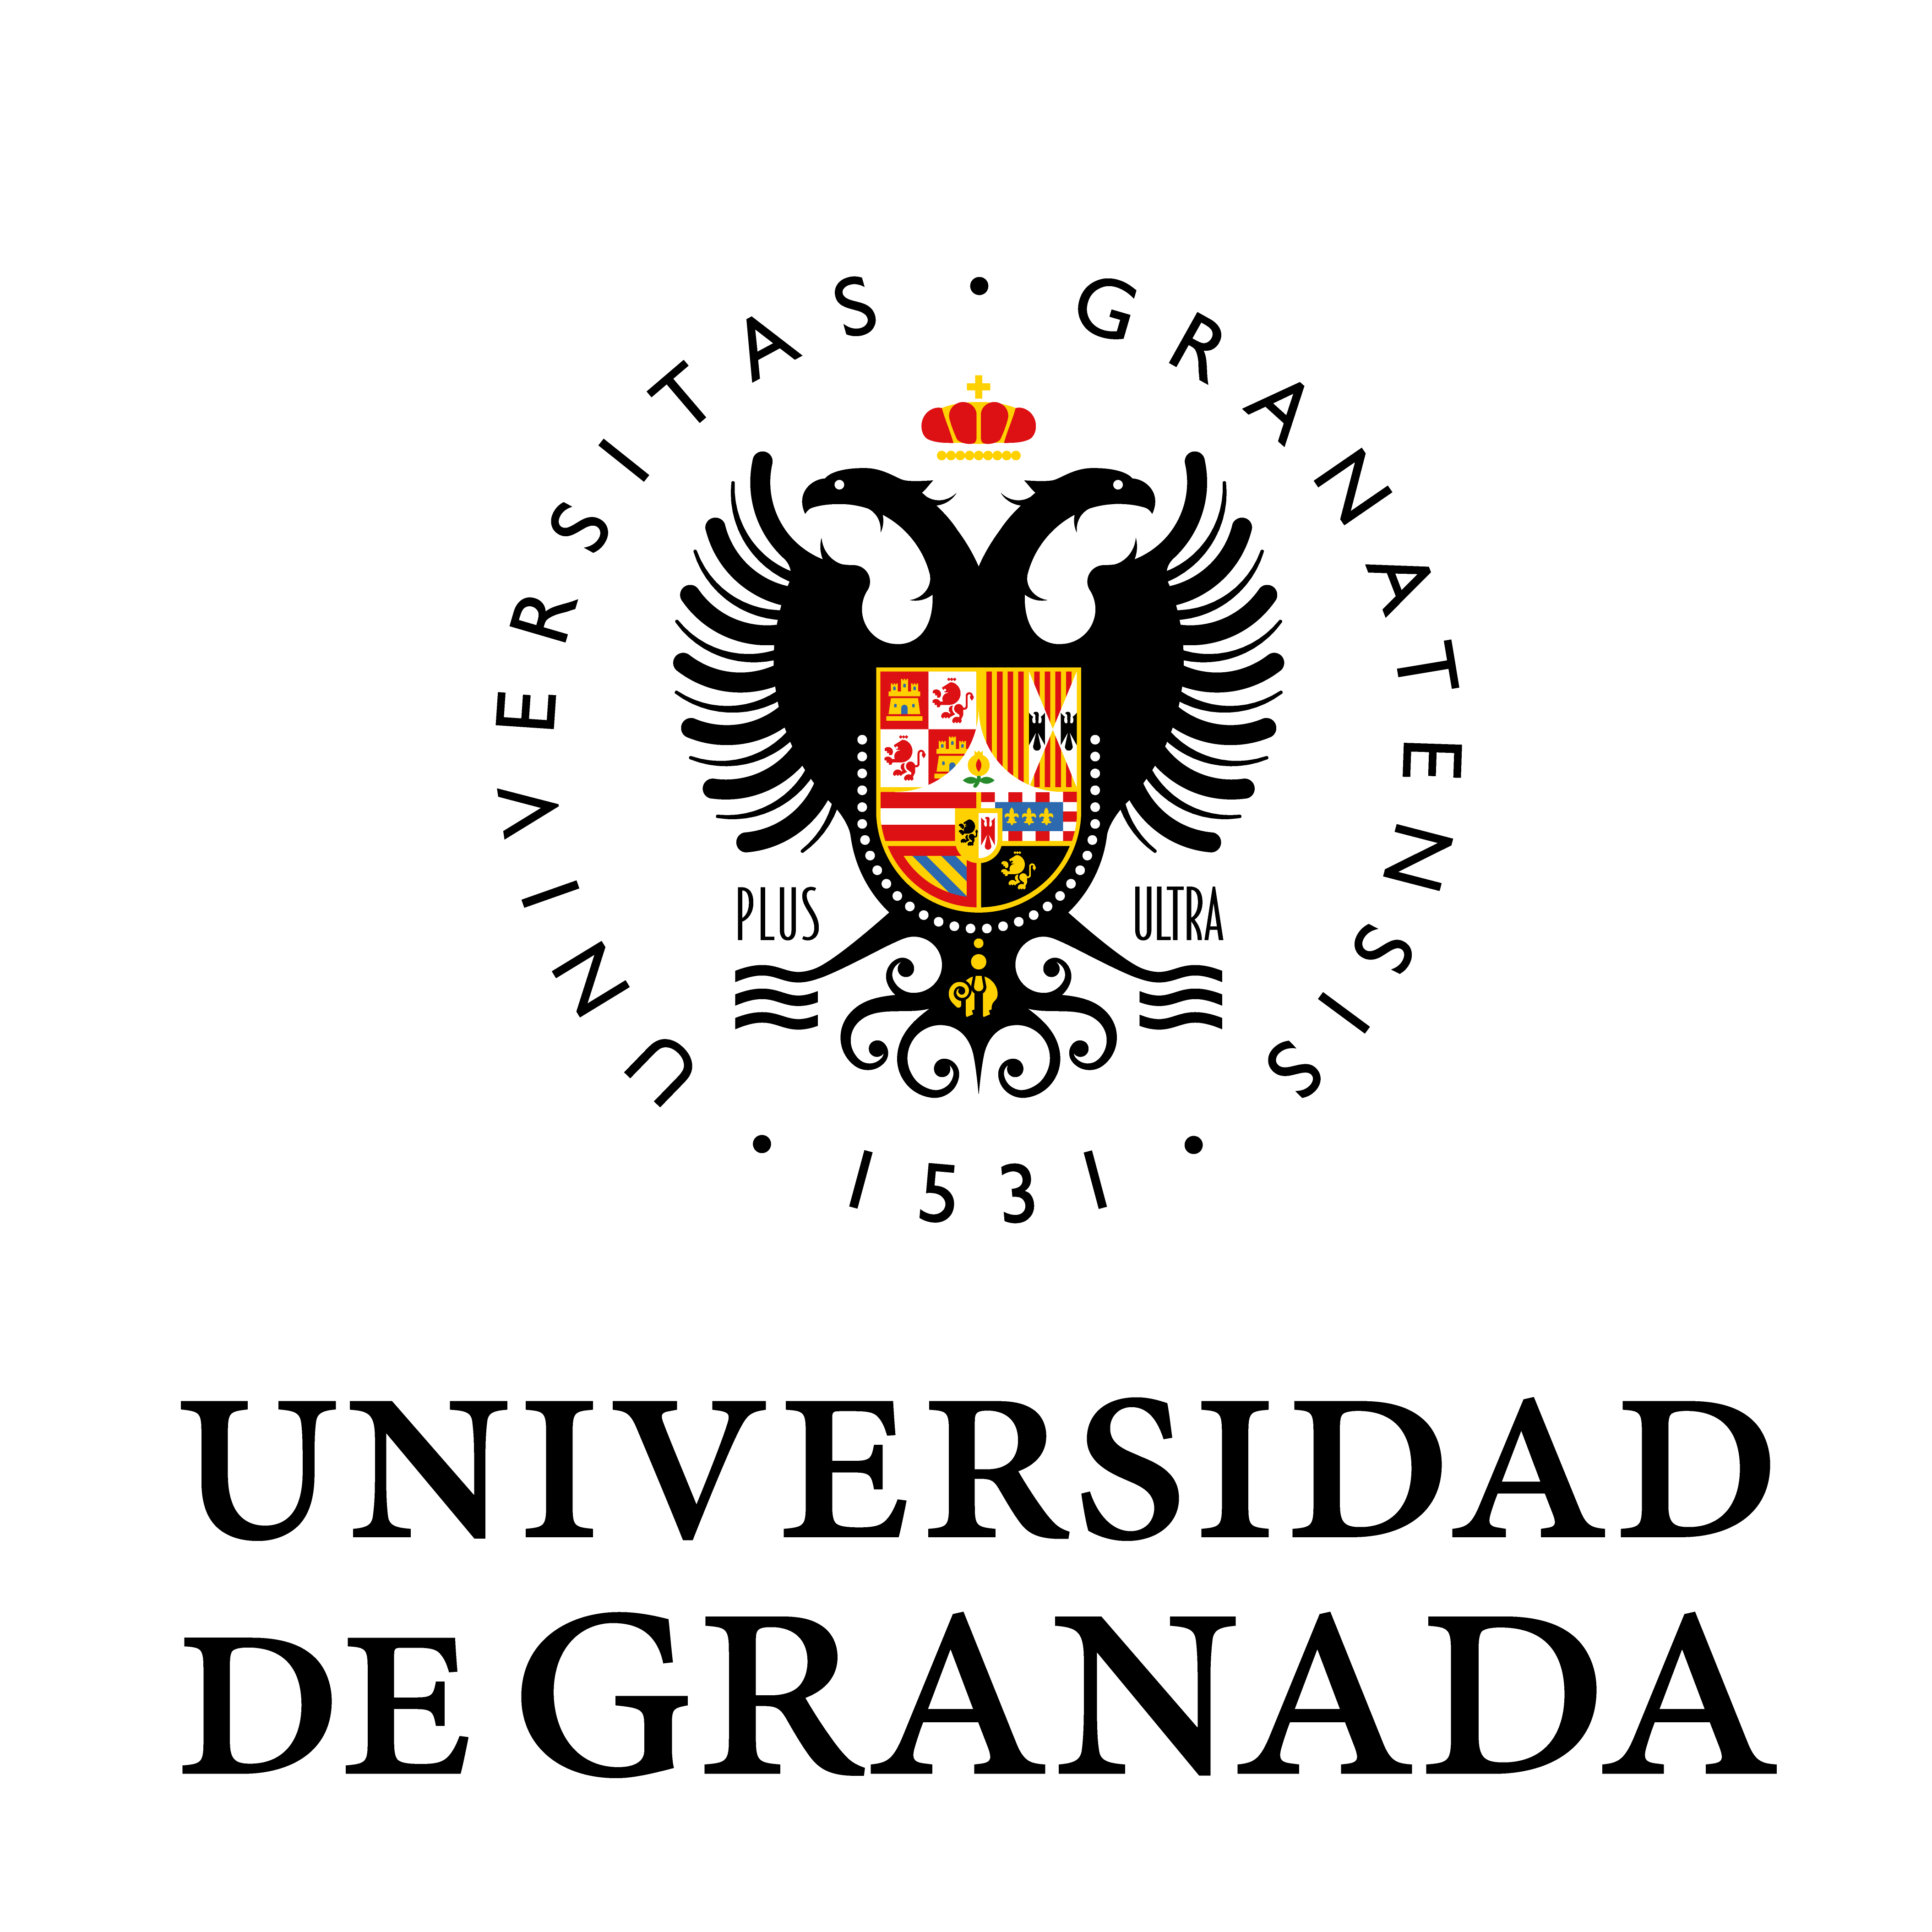
\includegraphics[width=0.9\textwidth]{./imagenes_memoria/ugr.png}\\[0.5cm]

\textsc{ \Large Práctica 1\\[0.2cm]}
\textsc{ \Large Ángel Cabeza Martín}\\
\textsc{ \Large 75571222F}\\
\textsl{ angelcabeza@correo.ugr.es}\\[0.5cm]
% Upper part of the page
% 
% Title
{\Huge\bfseries Máscaras y Derivadas\\
}
\noindent\rule[-1ex]{\textwidth}{2pt}\\[3.5ex]
{\large\bfseries Visión por Computador}
\end{titlepage}

%%%%%%%%%%%%%%%%%%%%%%%%%%%%%%%%%%%%%%%%%%%%%%%%%%%%%

\tableofcontents
\pagebreak
%%%%%%%%%%%%%%%%%%%%%%%%%%%%%%%%%%%%%%%%%%%%%%%%%%%%%

\section*{Introducción}
En esta práctica trabajaremos los filtros de máscaras, con el objetivo de extraer información significativa de imágenes y aprender el uso de las distintas propiedades de la función Gaussiana.\newline 

Esta práctica se centra en comparar nuestra implementación, hecha siguiendo la teoría, con la de OpenCV que se centra en buscar el máximo rendimiento obteniendo a su vez resultados aceptables, por ello todos los ejercicios estarán implementados sin usar ninguna función de OpenCV y solo usaremos estas por motivos comparativos.\\


Por último, quiero aclarar que en esta memoria no me voy a centrar en explicar cómo he desarrollado mi código, si no en las decisiones que he tomado para desarrollar la práctica y los conceptos teóricos que me han guiado para tomar esas decisiones.


\section{Ejercicio 1: Máscaras}
Este ejercicio trata sobre el cálculo de las máscaras Gaussianas que usaremos durante toda la práctica, la aplicación de estas para realizar una convolución y  para calcular un filtro Laplaciano y también aprenderemos cómo calcular máscaras a partir del kernel binomial. Además durante todos los apartados haremos una comparación entre nuestra implementación y la de OpenCV.

\subsection{Máscaras Discretas 1D}
Para calcular las distintas máscaras he implementado tres funciones:
\begin{enumerate}
	\item Función Gaussiana: Devuelve el valor de la función Gaussiana en un punto concreto para un sigma dado.
	\item Primera derivada de la función Gaussiana: devuelve el valor de la primera derivada de la Gaussiana para un punto concreto y un sigma dado
	\item Segunda derivada de la función Gaussiana: devuelve el valor de la segunda derivada de la Gaussiana para un punto concreto y un sigma dado
\end{enumerate}

Para la implementación de estas funciones, cogemos la expresión de la Gausiana y evaluamos el punto dado (he obviado la constante $c$ porque no influye en el cálculo):

\pagebreak

\begin{figure}
	\centering
	\[f(x) = c \cdot e^{-\frac{x²}{2\sigma²}} \]
	\caption{Función Gaussiana.}
	\label{f_gaussiana}
\end{figure}


Y para las derivadas simplemente hay que calcular las distintas derivadas de esta función respecto de $x$: 

\begin{figure}[H]
	\centering
	\[f'(x) = -\frac{x e^{-\frac{x²}{2 \cdot \sigma²}}}{\sigma²} \]
	\caption{Primera derivada de la Gaussiana.}
	\label{1d_gaussiana}
\end{figure}

\begin{figure}[H]
	\centering
	\[f''(x) = \frac{(x² - \sigma²) \cdot e^{-\frac{x²}{2*\sigma²}}}{\sigma⁴} \]
	\caption{Segunda derivada de la Gaussiana.}
	\label{2d_gaussiana}
\end{figure}

Una vez implementadas estas funciones, he creado la función \texttt{kernelGaussiano1D} que recibe como argumentos la función gaussiana a evaluar (por defecto sin derivada),un sigma y un tamaño de máscara. Estos dos últimos parámetros son opcionales pero siempre se tiene que dar por lo menos uno de ellos, si no el programa te advertirá de esto y parará. Si se proporciona únicamente uno de ellos, el otro se calcula con la fórmula de \ref{f_sigma_tam}. \\

Una vez calculado el sigma o el tamaño de la máscara, evaluaremos la función pasada como argumento (la Gaussiana, la 1º derivada de la Gaussiana o la 2º derivada de la Gaussiana) en el intervalo [-T//2,T//2] y, si la función usada es la Gaussiana, normalizaremos la máscara diviendo cada valor de la máscara entre la suma de todos los valores de la máscara.

\begin{figure}[H]
	\centering
	\[ 2 \cdot [3 \cdot \sigma] + 1 = T \]
	\caption{Fórmula para calcular sigma y T}
	\label{f_sigma_tam}
\end{figure}

Utilizamos esta fórmula ya que nos asegura que el tamaño de la máscara es al menos $3 \cdot \sigma$ y que dado un sigma este tamaño es impar. Ambas situaciones vimos en teoría que eran convenientes.

Tras calcular las máscaras de tamaño 5,7 y 9 y comparar los resultados con las máscaras calculadas por la función \texttt{getDerivKernel} de OpenCV hemos obtenido los resultados de las figuras \ref{mask_1d_t5} \ref{mask_2d_t5} \ref{mask_1d_t7} \ref{mask_2d_t7} \ref{mask_1d_t9} \ref{mask_2d_t9}. Como vemos las máscaras no son iguales, observamos dos grandes diferencias:

\begin{enumerate}
	\item Las máscaras de la primera derivada están invertidas.
	\item Cuanto mayor es el tamaño de la máscara, menor es el rango de valores en nuestras máscaras y mayor en las máscaras de getDerivKernels.
\end{enumerate}

La primera diferencia no es importante porque las máscaras son simétricas por lo que ambas máscaras suman 0. La segunda derivada se debe a que OpenCV no efectúa un kernel Gaussiano como tal, hace una aproximación usando los operadores Sobel o Scharr. Por lo tanto, nuestras máscaras son más exactas pero las de OpenCV son computacionalmente más rápidas.


\begin{figure}[H]
	\centering
	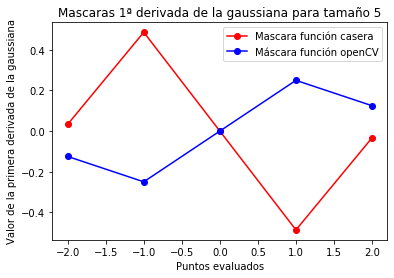
\includegraphics[width=12cm, scale=1]{./imagenes_memoria/1d_t5.png}
	\caption{Comparativa de las máscaras de 1ª derivada de tamaño 5 de getDerivKernels y nuestra función}
	\label{mask_1d_t5}
\end{figure}

\begin{figure}[H]
	\centering
	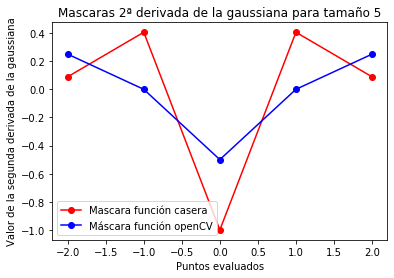
\includegraphics[width=12cm]{./imagenes_memoria/2d_t5.png}
	\caption{Comparativa de las máscaras de 2ª derivada de tamaño 5 de getDerivKernels y nuestra función}
	\label{mask_2d_t5}
\end{figure}

\begin{figure}[H]
	\centering
	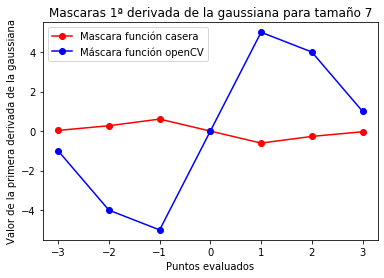
\includegraphics[width=12cm]{./imagenes_memoria/1d_t7.png}
	\caption{Comparativa de las máscaras de 1ª derivada de tamaño 7 de getDerivKernels y nuestra función}
	\label{mask_1d_t7}
\end{figure}

\begin{figure}[H]
	\centering
	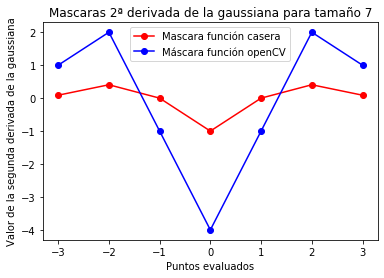
\includegraphics[width=12cm]{./imagenes_memoria/2d_t7.png}
	\caption{Comparativa de las máscaras de 2ª derivada de tamaño 7 de getDerivKernels y nuestra función}
	\label{mask_2d_t7}
\end{figure}

\begin{figure}[H]
	\centering
	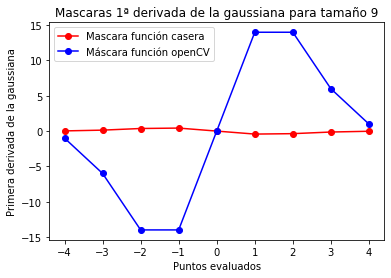
\includegraphics[width=12cm]{./imagenes_memoria/1d_t9.png}
	\caption{Comparativa de las máscaras de 1ª derivada de tamaño 9 de getDerivKernels y nuestra función}
	\label{mask_1d_t9}
\end{figure}

\begin{figure}[H]
	\centering
	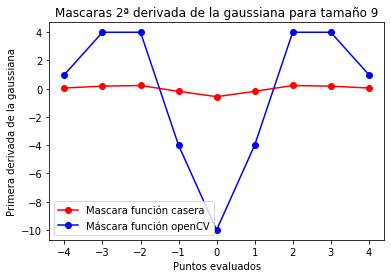
\includegraphics[width=12cm]{./imagenes_memoria/2d_t9.png}
	\caption{Comparativa de las máscaras de 2ª derivada de tamaño 9 de getDerivKernels y nuestra función}
	\label{mask_2d_t9}
\end{figure}

\subsection{Kernel binomial}
En este ejercicio se nos pide calcular las máscaras de tamaño 5 y 7, tanto de alisamiento como de derivada, a partir de la aproximación binomial de la Gaussiana ([1,2,1]) y la máscara de derivada de orden 3 ([-1,0,1]. //

Para hacer esto

\subsection{Convolución}
En este ejercicio se nos pide realizar una convolución en 2D, a partir de dos máscaras 1D. Para ello he implementado las siguientes funciones:

\begin{itemize}
	\item aniadeborde: Recibe como argumentos una imágen y la máscara con la que se va a convolucionar. Esta función hace uso del método CopyMakeBorder de OpenCV para añadir un borde con un tamaño igual a la mitad de la longitud de la máscara.
	\item convolucionar: esta función recibe una imágen (con el borde ya añadido) y dos máscaras, una con la convolucionar por filas y otra por columnas (lo he hecho así porque me facilitaba el siguiente ejercicio pero realmente se podría hacer con una sola) y devuelve la imagen convolucionada.
	\item Además me he servido de las funciones creadas en la práctica 0 para leer imágenes, dibujarlas etc...
\end{itemize}

Para hacer la convolución he seguido este esquema:

\begin{itemize}
	\item Calcular el tamaño del borde que se ha añadido a la imágen para saber dónde empieza la imágen original. Esto se hace dividiendo el tamaño de la máscara entre dos.
	\item Calcular el tamaño de la imagen original (la imágen sin bordes) restando a la dimensión de la imagen actual el doble del borde calculado en el paso uno, ya que este borde se añade dos veces por filas y dos veces por columnas.
	\item Crear una matriz con las dimensions calculadas en el paso anterior. Esta matriz será el resultado de hacer la convolución sobre la imagen
	\item Recorrer la imágen con bordes pero sin contar con ellos, es decir, recorrer la imagen desde el tamaño del borde hasta el extremo de la imagen menos el borde. De esta forma recorremos toda la imagen original, centrando la máscara en el pixel que estemos recorriendo y multiplicando esta por los pixeles de una misma fila, pero tantos como sea el tamaño de la máscara. El resultado de esta operación se almacena en la matriz creada en el paso 3.
	\item Tras aplicar la máscara de manera horizontal, le añadimos los bordes nuevamente a la imagen obtenida, para aplicar la máscara de manera vertical y que la imágen no disminuya en tamaño.
	\item Repetimos el paso 4 pero por columnas,es decir, mantenemos la columna y escogemos un rango de pixeles en las filas para aplicar la máscara vertical.
	\item Devolvemos la imágen generada.
\end{itemize}

Hay que destacar que me he servido de la propiedad de separabilidad  para poder aplicar primero la máscara 1D por filas y luego por columnas. Si la Gaussiana no tuviese esta propiedad, no sería posible realizar la convolución de esta manera. \\

Una vez implementada la convolución, vamos a comparar los resultados que obtenemos nosotros con los que se obtienen usando la función de OpenCV GaussianBlur con una mácara de tamaño 9:

\begin{figure}[H]
	\centering
	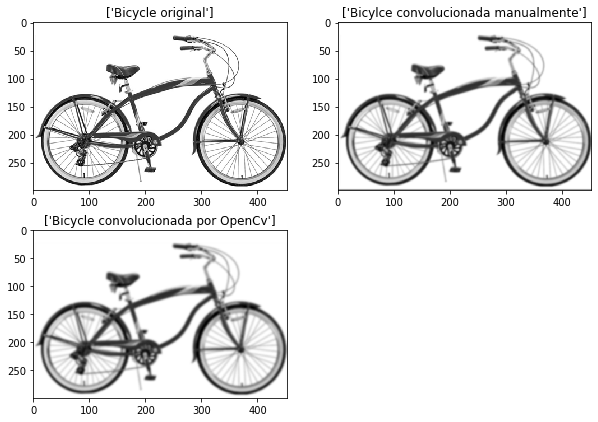
\includegraphics[width=\textwidth]{./imagenes_memoria/bycicle_bifuminada.png}
	\caption{Comparación entre convolución propia (a la derecha) y GaussianBlur (abajo izuierda)}
	\label{conv_propia_vs_openCV}
\end{figure}

Como vemos la diferencia entre nuestra convolución y la de OpenCV es mínima, por lo tanto podemos asumir que la convolución está implementada de manera correcta. La diferencia que hay se puede deber a que como vimos anteriormente OpenCV calcula las máscaras de manera distinta a como lo hacemos nosotros.

\pagebreak

Tras haber convolucionado con una máscara de suavizado la imágen, vamos a hacerlo con las máscaras de derivadas y obtenemos lo siguiente:

\begin{figure}[H]
	\centering
	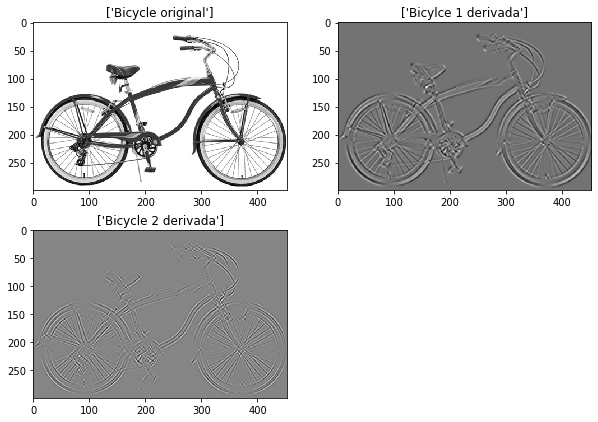
\includegraphics[width=\textwidth]{./imagenes_memoria/bycicle_derivadas.png}
	\caption{Imagén convolucionada con la primera derivada (a la derecha) y con la segunda derivada (abajo izquierda}
	\label{conv_1y2d_bycicle}
\end{figure}

Como vemos obtenemos el resultado esperado ya que hemos usado las derivadas de la Gaussiana que son filtros de detección de bordes y es justo lo que observamos en la imágen.

\subsection{Máscara Laplaciana}
En este ejercicio se nos pide calcular la máscara Laplaciana a partir de una Gaussiana y comparar los resultados con la función Laplaciana de OpenCV. \\

Como sabemos, la máscara Laplaciana es la suma de la convolución por filas con la derivada segunda de la Gaussiana y, luego, por columnas, la convolución con la Gaussiana más la convolución por filas con la Gaussiana y, luego, por columnas, la convolución con la derivada segunda de la Gaussiana y todo por $\sigma²$ (\ref{f_laplaciana} para verlo de forma matemática).

\begin{figure}[H]
	\centering
	\[L = \sigma² \cdot (G_{xx}(x,y,\sigma) + G_{yy}(x,y,\sigma)) \]
	\caption{Función Gaussiana.}
	\label{f_laplaciana}
\end{figure}

Por este motivo, de cara a calcular la imagen con la máscara Laplaciana aplicaremos una convolución de la imágen con la máscara de la segunda derivada de la Gaussiana por filas y la máscara Gaussiana por columnas, a esto lo llamaremos $dxx$. Después aplicaremos una convolución a la imágen original con la máscara Gaussiana por filas y la máscara de la segunda derivada de la Gaussiana por columnas, a esto lo llamaremos $dyy$. Finalmente multiplicaremos por $\sigma²$ la suma de $dxx$ y $dyy$ y esta será la máscara Laplaciana que devolveremos. \\

Y, calculando la máscara Laplaciana como hemos comentado, obtenemos los siguientes resultados: 

\begin{figure}[H]
	\centering
	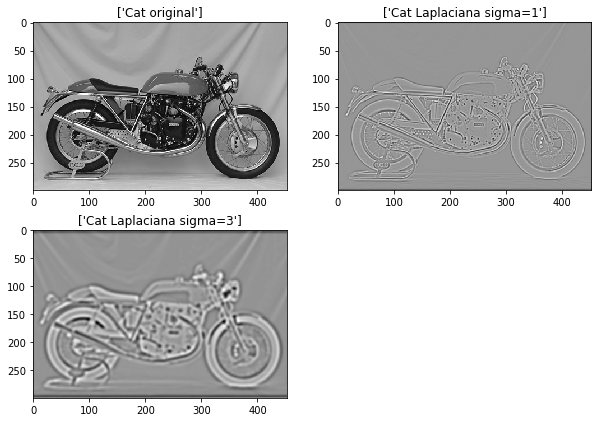
\includegraphics[width=\textwidth]{./imagenes_memoria/motocicleta_laplaciana.png}
	\caption{Comparación de imágenes tras aplicar la máscara Laplaciana con distinto $\sigma$)}
	\label{comp_sigma_laplaciana}
\end{figure}

\end{document}
